\begin{figure}[p]
	\begin{center}
		\fbox{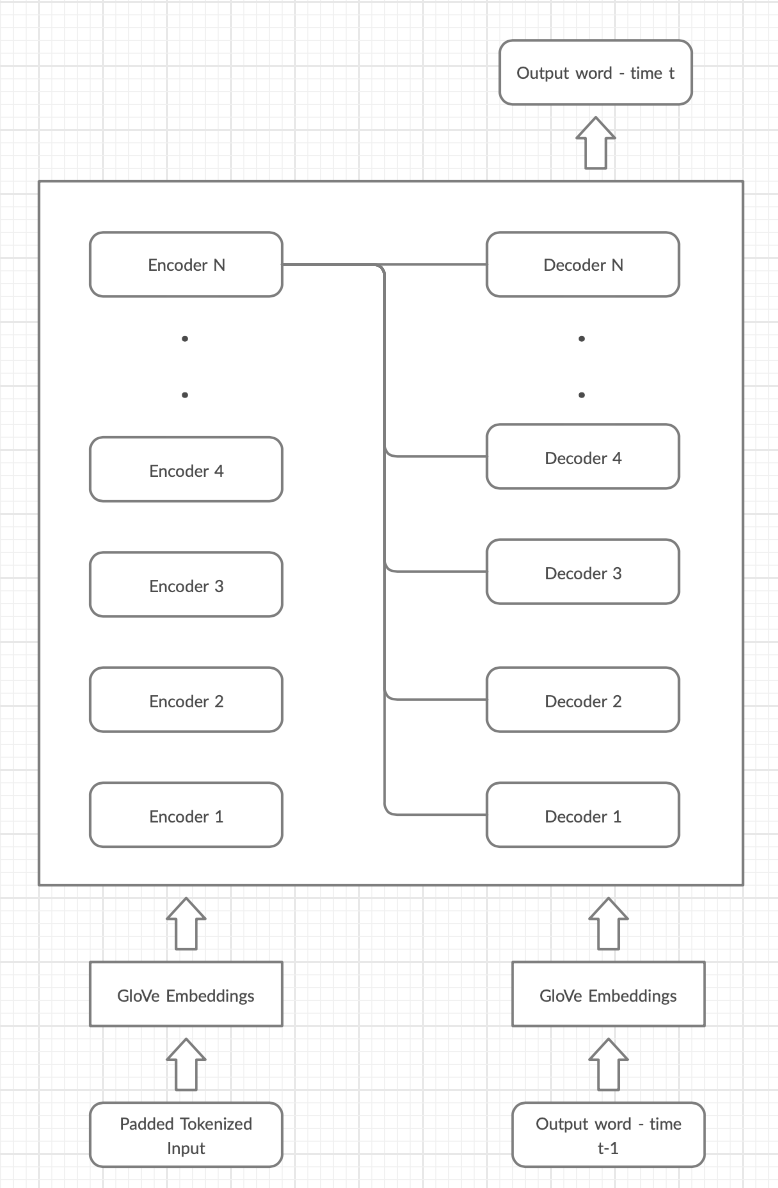
\includegraphics[width=1\textwidth]{TransformerImage.png}}
	\end{center}
	\caption{Transformer based Seq2Seq model.}
	\label{fig:trans_model_image}
\end{figure}

The second model we considered was another sequence-to-sequence model that used \emph{transformers} (See Figure \ref{fig:trans_model_image}).
The introduction of {transformers} in 2017 and it's success in \emph{natural language processing} tasks have caused it to replace LSTM \cite{DBLP:journals/corr/VaswaniSPUJGKP17}. 
The transformer performs better in retaining long-range context dependencies. 
It works on the self-attention mechanism. 
The recent performances of Google BERT (trained using transformers) and transformers in general motivated us to try it in our task.
In this section we discuss how we developed, trained and analyses this model.

\subsection{Model Architecture}

The Embedding layer uses the \emph{subword text encoder} from the Tensorflow datasets library. 
The architecture as shown in Figure \ref{fig:trans_model}, shows the structure of a single encoder-decoder unit. 
The units are designed such that the outputs of each encoder is connected to every decoder. 
The number of such units is a hyper-parameter.

The internal structure of the encoder contains a multi-head attention mechanism and a feed-forward network (See Figure \ref{fig:attention}). 
The multi-head attention network computes a series of scalar dot product attentions in parallel. 
This produces a base for enabling self-attention and sort of acts like an ensemble technique. 
The self-attention is computed using three vectors - \emph{query}, \emph{key} and \emph{value}. 
The weights for these vectors are learned during training. 
The dot product between each word embedding vector and each of these keys are used to compute self-attention. 
This process is done in parallel, multiple times. 
These outputs are concatenated and sent to the feed-forward network. 
The above process allows to jointly attend to information from different sub-spaces of representation.

The internal structure of the decoder is similar to the sub components of the encoder. 
The difference is the addition of a masked multi-head encoder. 
It is similar to the multi-head attention with a masking layer. 
The query vector to a decoder comes from the previous decoder layer while the key and value vectors come from the encoder network layers. The query, key and value vectors for the encoder units come from previous encoder layers. 
The decoder outputs from the feedfoward network is softmaxed over the vocabulary to produce the next probable word.

\begin{figure}[ht]
  \centering
  \begin{minipage}[b]{0.40\textwidth}
    \begin{center}
		\fbox{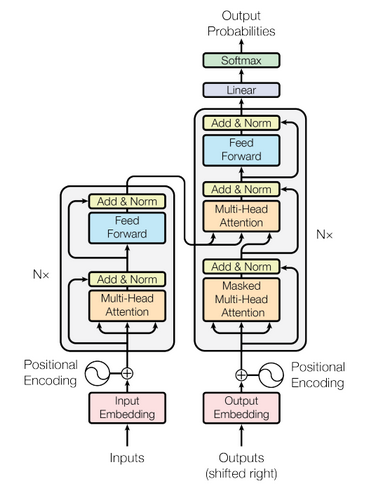
\includegraphics[width=\textwidth]{transformer.png}}
	\end{center}
    \caption{Encoder Decoder Unit. Image taken from \cite{DBLP:journals/corr/VaswaniSPUJGKP17}}.
    \label{fig:trans_model}
  \end{minipage}
  \hfill
  \begin{minipage}[b]{0.40\textwidth}
    \begin{center}
		\fbox{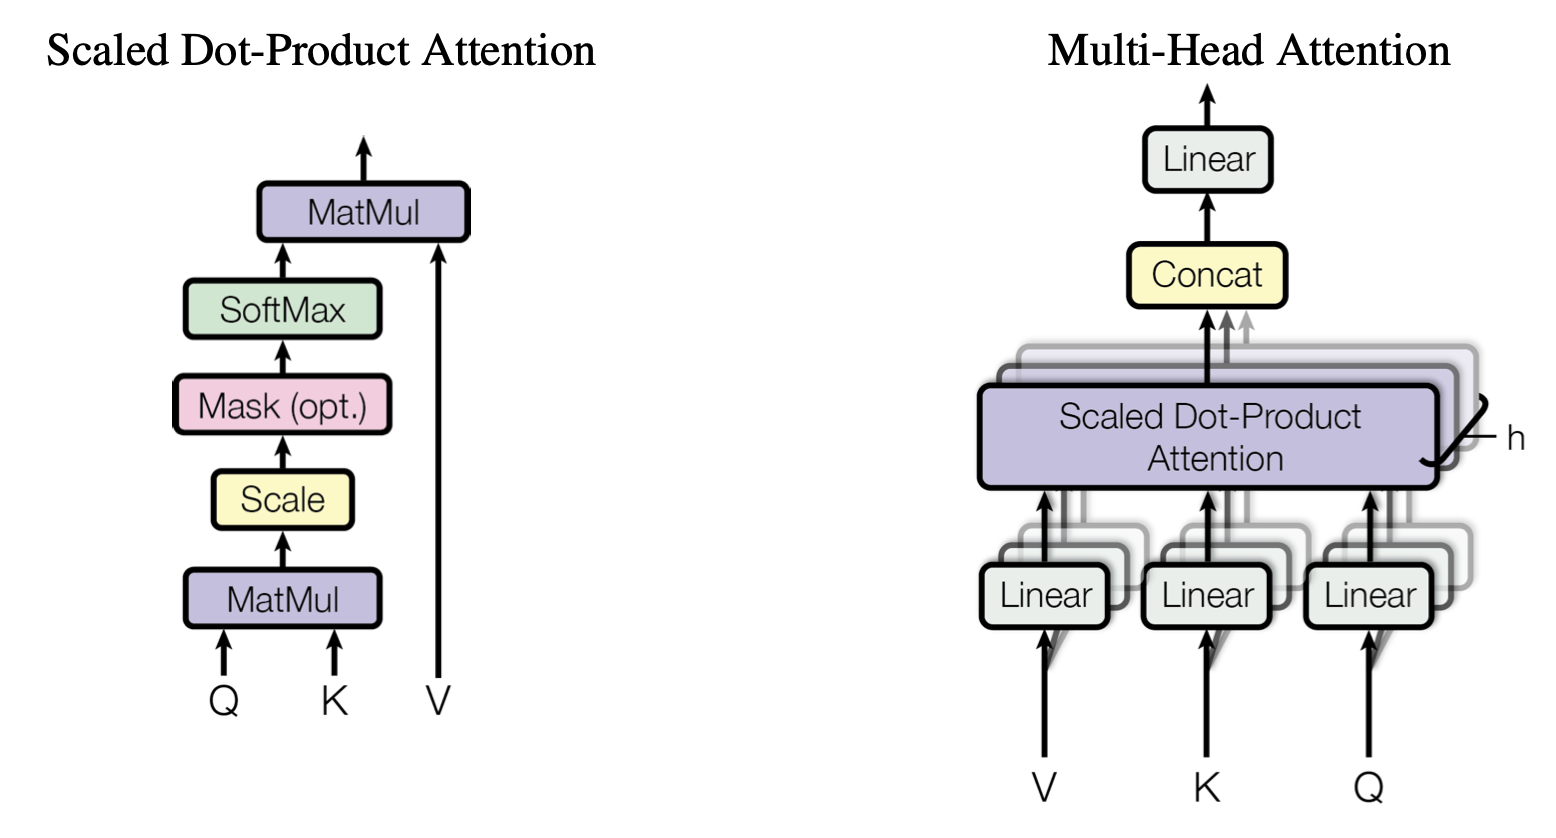
\includegraphics[width=\textwidth]{attention.png}}
	\end{center}
    \caption{Attention mechanism. Image taken from \cite{DBLP:journals/corr/VaswaniSPUJGKP17}}
    \label{fig:attention}
  \end{minipage}
\end{figure}

\subsection{Performance and Error Analysis}
\label{subsec:trans_s2s}
\begin{figure}[ht]
	\begin{center}
		\scalebox{.8}
		{
			\begin{tabular}{ |l|c|c|c|c|c|c|c| } 
				\hline
				\textbf{Dataset} & \textbf{BLEU Avg. Score} & \textbf{ROUGE-1 Score} & \textbf{ROUGE-$\ell$} & \textbf{METEOR Score} & \textbf{WER Avg.} & \textbf{Human Eval.}\\
				\hline
				Q\&A & $0$ & $0.102$ & $0.094$ & $0,035$ & $2.412$ & $0.263$\\
				\hline
				Joey & $0.110$ & $0.270$ & $0.0.261$ & $0.137$ & $1.218$ & $0.325$\\ 
				\hline
			\end{tabular}
		}
	\end{center}
	\caption{Table showing various scores for this sequence-to-sequence model with transformers on the Joey and generic questions and answers dataset (Q\&A).}
	\label{fig:trans_res}
\end{figure}
We note that the automatic metrics were run using our final trained models.
That is, we ran all the experiments  with a model trained first on the generic dataset and then the Joey dataset.
Based on the test results, both human and automatic metrics, the transformer model works better on the Joey dataset compared to the generic dataset.
One theory as to why this happened is that the transformer model performs better on datasets with large vocabulary and the generic questions and answer dataset has a very small vocabulary.
Moreover, we suspect that small size of the generic dataset compared to the Joey dataset may have been a big factor as well.

As we discussed in the previous section, considering a larger generic dataset may produce more promising results in final performance.
Just like the first sequence-to-sequence model, this model consistently generated response that did not parse as proper English sentences. 
%A review of the outputs produced on the generic test set will show that while responses are very different from the test response, they are still close just as close to English sentences (if not closer) compared to the original sequence-to-sequence model.
Future work could include trying to work on mapping how the model constructs a generic response and then tries to add 'Joey' characteristics to it. 
%Training the model on multiple datasets did not seem to solve this problem. 
We would suggest trying to add an additional learned component that tries to implement the idea of adding characteristics.
%Based on our initial test trials, we realized that the model is learning to respond based on a corpus entirely composed of the character's responses and has limited understanding of sentence formation. 
%Training the model on a general question answering corpus did not significantly increase the quality of sentences.
Therefore, a possible improvement to our model would be to train the model on a \emph{part of sentence task}. 
This might enable the model to learn sentence formulation mappings and could structure the sentences better.
%
%The Transformer model performs significantly better when the questions overlap contexts present in the television show. 
%The model generates responses that has fewer 'Joey' characteristics when asked generic questions than when asked questions with overlapping TV show context. 
%Overcoming this could be possible with the Part of Sentence training.

\subsection{Pitfalls and Improvements}
Some of the major roadblocks we faced during our implementation of this model included the construction of the transformer. 
There were no Keras or Tensorflow/PyTorch implementation of a basic transformer. 
Therefore, we had to refer to other sources to provide us with an implementations of the multi-head attention and positional encoding \cite{transmedium}. 

Another issue we faced was the inclusion/construction of context.
We tried to include the entire chat history (sequence of sentences processed previously) as a context vector to each computation. 
However, this idea did not increase the quality of results in \cite{DBLP:journals/corr/VaswaniSPUJGKP17} because the compilation of the entire history/context into a single vector doesn't seem to be effective. 
Therefore, we worked on producing output responses independent of previous context. 
Other sources (\cite{learndesmedium} and \cite{chatbotmedium}) indicate using the concept of goals/entities where the chatbot would recognize certain parts of the conversation as required entities (stored as context) and would work towards reaching a goal. 
This approach is quite specific and does not apply to general chatbots. 
We recognize this task as a possible area for future improvement.
